We must select a downstream region for which to look for a heavy photon having virtually no background. Therefore, we choose a $zCut$ which is a downstream z vertex position beyond which there is less than 0.5~background event/bin. We arbitrarily choose our maximum z value, $zMax$, to be at the first layer, although this can vary depending on the dataset. The $zCut$ varies as a function of mass and can be ideally selected to minimize backgrounds whilst maximizing A' production. The number of events we can expect to reconstruct is described by Equation~\eqref{eq:signal}.

\begin{equation}
\label{eq:signal}
S_{bin,zCut} = \left( \dfrac{N_{rad}}{N_{tot}}\right) N_{bin}\left(\dfrac{3\pi\epsilon^{2}}{2N_{eff}\alpha}\right)\left(\dfrac{m_{A'}}{\delta m_{A'}}\right)\epsilon_{bin}\int_{zCut}^{zMax}\dfrac{e^{-ztgt-z/\gamma c\tau}}{\gamma c \tau}\epsilon_{vtx}(z,m_{A'})dz
\end{equation}

In Equation~\eqref{eq:signal}, the heavy photon production at the target per mass bin is described by the first four terms. $\epsilon_{bin}$ is chosen as the fraction of signal we reconstruct within our selected mass bin window(we choose a mass window of $\pm1.4\sigma_m$ corresponding to an $\epsilon_{bin}$ of 0.838). The $N_{rad}/N_{tot}$ is the radiative fraction which is the fraction of radiatives contained in the sample and is derived from Monte Carlo. The $N_{bin}$ is the number of measured e+e- pairs at a given mass. The third and fourth terms are what was explained in Equation~\eqref{eq:crossSection}. The integral calculates the number of heavy photons we could reconstruct in the decay region from $zCut$ to $zMax$, where $z=0$ is the target location. $\epsilon_{vtx}$ represents the efficiency of detecting $e+e-$ pairs from an A' of mass $m_{A'}$ that decayed at position $z$ from the target and is inclusive of the efficiencies of all other cuts used in the analysis. Based on Poisson statistics, the 90$\%$ confidence limit for a null result requires to have an expected number of A' events as defined in Equation~\ref{eq:signal} to be greater than 2.303.\\
\indent In order to find the value of $zCut$, we slice the distribution of the reconstructed vertex position versus reconstructed mass in bins of mass and fit the core of the vertex distribution with a Gaussian with the normal parameters of $\sigma$ and $z_{mean}$ while fitting the downstream tail of the distribution with an exponential. The fit for the full vertex distribution per mass bin is described by Equation~\eqref{eq:vtxFit}.

\begin{eqnarray*}
\label{eq:vtxFit}
F(z < b) & = & Ae^{-\dfrac{(z-z_{mean})^2}{2\sigma^2}}\\
F(z > b) & = & Ae^{-\dfrac{b^2}{2\sigma^2}-\dfrac{z-z_{mean}-b}{l}}\\
\end{eqnarray*}

As shown in Equation~\eqref{eq:vtxFit}, there is an additional parameter $b$ which defines the distance from the core of the Gaussian that the fit will be described by the exponential tail. The exponential tail, where $z>b$, is defined in terms of the parameter $l$, controlling the length of the tail, and describes the downstream tail of the vertex distribution. The $zCut$ is selected from this function where there remains 0.5 background events downstream. A fit to a mass slice from the L1L1 dataset is shown in Figure~\ref{fig:vtxFitPic}.

\begin{figure}[H]
  \centering
      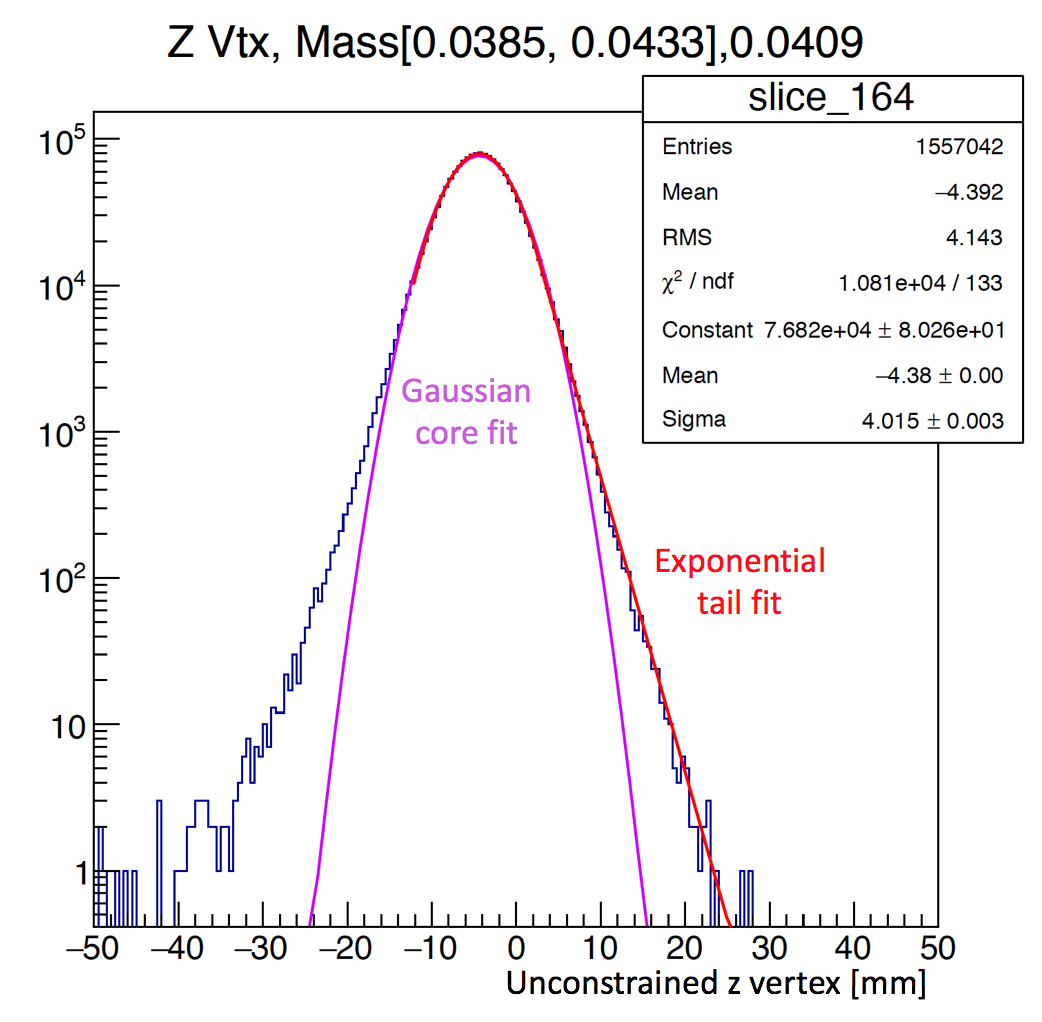
\includegraphics[width=0.8\textwidth]{pics/searching/vtxFit.png}
  \caption{For a mass slice centered at 31~MeV, the vertex distribution in the L1L1 dataset is shown and fitted. The fit functions are described by Equation~\eqref{eq:vtxFit} where the core of the distribution is fit with a Gaussian and the downstream tail is fit with an exponential.}
  \label{fig:vtxFitPic}
\end{figure} 

